\documentclass[11pt,a4paper,openany]{report}

\usepackage[margin=2.5cm]{geometry}
\usepackage[T1]{fontenc}
\usepackage[utf8]{inputenc}
\usepackage{lmodern}
\usepackage{microtype}
\usepackage{xcolor}
\usepackage{graphicx}
\usepackage{eso-pic}
\usepackage{amsmath,amssymb}
\usepackage{booktabs}
\usepackage{tabularx}
\usepackage{longtable}
\usepackage{array}
\usepackage{enumitem}
\usepackage{listings}
\usepackage{float}
\usepackage{tikz}
\usetikzlibrary{arrows.meta,positioning,shapes.geometric,shapes.multipart,fit,calc,backgrounds,decorations.pathreplacing}
\usepackage{fancyhdr}
\usepackage{titlesec}
\usepackage{hyperref}
\Urlmuskip=0mu plus 1mu
\usepackage{caption}

\definecolor{PolimiBlue}{RGB}{0,83,155}
\definecolor{LightBlue}{RGB}{232,242,250}
\definecolor{LightGray}{RGB}{246,246,246}
\definecolor{DarkGray}{RGB}{70,70,70}

\hypersetup{
  colorlinks=true,
  linkcolor=PolimiBlue,
  citecolor=PolimiBlue,
  urlcolor=PolimiBlue,
  pdftitle={Requirements Analysis and Specification Document - UAV Test Generator},
  pdfauthor={Roberto Capone and Guglielmo Cattaneo}
}

\setcounter{tocdepth}{3}
\setcounter{secnumdepth}{3}
\setlist[itemize]{leftmargin=1.6em,itemsep=2pt,topsep=4pt}
\setlist[enumerate]{leftmargin=1.8em,itemsep=2pt,topsep=4pt}
\renewcommand{\arraystretch}{1.18}
\newcolumntype{Y}{>{\raggedright\arraybackslash}X}
\newcolumntype{L}[1]{>{\raggedright\arraybackslash}p{#1}}

\pagestyle{fancy}
\fancyhf{}
\fancyhead[L]{UAV Test Generator -- Requirements Analysis and Specification}
\fancyhead[R]{Version 1.0}
\fancyfoot[C]{\thepage}
\setlength{\headheight}{14pt}

\titleformat{\chapter}[display]
  {\normalfont\bfseries\color{PolimiBlue}}
  {\filleft\Large\chaptertitlename\ \thechapter}
  {1ex}
  {\titlerule\vspace{1ex}\filright\Huge}

\lstset{
  basicstyle=\ttfamily\small,
  backgroundcolor=\color{LightGray},
  frame=single,
  rulecolor=\color{black!20},
  breaklines=true,
  columns=fullflexible,
  keepspaces=true,
  showstringspaces=false
}

\newcommand{\projecttitle}{Search-Based Test Generation for Autonomous UAV Obstacle Avoidance Using a $(1+1)$-Evolution Strategy}
\newcommand{\systemname}{UAV Test Generator}
\newcommand{\req}[1]{\textbf{#1}}
\newcommand{\priorityM}{\textbf{Mandatory}}
\newcommand{\priorityS}{\textbf{Should}}
\newcommand{\priorityC}{\textbf{Could}}

\begin{document}
\raggedbottom

% ---------------------------------------------------------------------------
% Front page
% ---------------------------------------------------------------------------
\begin{titlepage}
\centering
\vspace*{0.55cm}

\includegraphics[width=0.32\textwidth]{polimi_logo.png}\par
\vspace{0.30cm}
{\large Software Engineering for Automation\par}
{\large A.Y. 2025--2026\par}
\vfill
{\Huge\bfseries\color{PolimiBlue} Requirements Analysis and Specification Document\par}
\vspace{0.8cm}
{\Large\bfseries \projecttitle\par}
\vfill
\begin{tabular}{rl}
\textbf{Authors:} & Roberto Capone\\
                  & Guglielmo Cattaneo\\[4pt]
\textbf{Instructor:} & Prof. Matteo Camilli\\[4pt]
\textbf{Version:} & 1.0\\
\textbf{Release date:} & 17/07/2026
\end{tabular}
\vfill
\end{titlepage}

\chapter*{Revision History}
\addcontentsline{toc}{chapter}{Revision History}
\begin{table}[H]
\centering
\begin{tabularx}{\textwidth}{L{2.2cm} L{2cm} L{4cm} Y}
\toprule
\textbf{Date} & \textbf{Version} & \textbf{Authors} & \textbf{Description}\\
\midrule
17/07/2026 & 1.0 & Roberto Capone; Guglielmo Cattaneo & Initial complete release aligned with the final \texttt{es-generator} implementation branch.\\
\bottomrule
\end{tabularx}
\end{table}

\tableofcontents
\clearpage

% ===========================================================================
\chapter{Introduction}
% ===========================================================================

\section{Purpose}
This document specifies the requirements of the \systemname, a search-based software testing tool developed for the UAV Testing Competition. The system generates challenging obstacle configurations for the autonomous obstacle-avoidance behaviour of PX4-Avoidance, executes the resulting tests through the Aerialist test bench, and returns an ordered suite of failing test cases.

The document has four objectives:
\begin{enumerate}
  \item define the system boundary and the relevant external actors;
  \item state functional and non-functional requirements in a verifiable form;
  \item describe the domain, principal scenarios, assumptions, dependencies, and constraints;
  \item provide requirements-level behavioural models to support the subsequent design and implementation documents.
\end{enumerate}

The intended audience consists of the project authors, the course instructor, maintainers of the generator, competition evaluators, and readers who need to verify consistency between requirements, design, implementation, and experimental results.

\section{Scope}
The \systemname is a command-line application that receives:
\begin{itemize}
  \item an Aerialist YAML case-study description containing the UAV configuration, mission plan, and simulation environment; and
  \item a positive integer defining the maximum number of simulation attempts available to the generator.
\end{itemize}

The system produces one or more test cases containing between one and three non-overlapping box-shaped obstacles. Candidate configurations are evaluated in simulation. A test is considered failing when the minimum distance between the UAV trajectory and at least one obstacle is below the safety threshold of $1.5\,\mathrm{m}$. The search objective is the continuous minimum distance, whereas the final delivery order additionally accounts for failure severity, number of obstacles, and execution time.

The implemented search method is a $(1+1)$-Evolution Strategy with adaptive mutation, restart, targeted obstacle insertion, persistent checkpointing, and failure diversity management. An independent random-search baseline is included for controlled experimental comparison.

The following elements are outside the system boundary and are not modified by this project:
\begin{itemize}
  \item PX4-Avoidance and the PX4 autopilot software;
  \item the Gazebo simulator and its physical models;
  \item the Aerialist execution framework;
  \item the official mission definitions and competition evaluator;
  \item the host operating system, Docker engine, and container runtime.
\end{itemize}

\section{Definitions, Acronyms, and Abbreviations}
\begin{longtable}{L{3.3cm} L{11.5cm}}
\toprule
\textbf{Term} & \textbf{Definition}\\
\midrule
\endfirsthead
\toprule
\textbf{Term} & \textbf{Definition}\\
\midrule
\endhead
Aerialist & Simulation-based UAV test bench that configures and executes PX4/Gazebo tests and returns flight logs.\\
Archive & Bounded in-memory collection of selected failing individuals used to construct the final delivery suite.\\
Candidate / Individual & One obstacle configuration together with its measured fitness, trajectory, completion flag, ranking data, and persistent artifact reference.\\
Case study & Input YAML description of a UAV mission and simulation environment without generated obstacles.\\
Checkpoint & Persistent JSON representation of the search state, sufficient to continue a run after process or simulator failure.\\
DTW & Dynamic Time Warping; a trajectory-alignment distance used by the implementation to identify similar failure behaviours.\\
ES & Evolution Strategy. The implemented search is a $(1+1)$-ES with one current parent and one generated child per iteration.\\
Failing test & A test for which the observed minimum UAV--obstacle distance is lower than $1.5\,\mathrm{m}$.\\
Fitness & Continuous search objective equal to the minimum UAV--obstacle distance observed for a candidate; lower values are better.\\
Genome & Ordered list of one to three obstacle genes. Each gene is $[l,w,h,x,y,r]$.\\
Hard fail & Collision or near-collision, operationally associated with a minimum distance close to zero.\\
IoU & Intersection over Union of two obstacle footprints. Used as a geometric fallback when trajectory data are unavailable and for restart novelty.\\
Operator & Human user who starts, monitors, or stops a generation campaign.\\
PX4-Avoidance & Vision-based autonomous obstacle-avoidance system under test.\\
SITL & Software-in-the-loop simulation.\\
Soft fail & Safety-distance violation with minimum distance below $1.5\,\mathrm{m}$, whether or not the mission is completed.\\
Test budget & Maximum number of simulation attempts that may be consumed by one generator run.\\
Test suite & Ordered set of generated test cases exported for evaluation.\\
ULog & PX4 flight-log format containing the recorded trajectory and telemetry.\\
YAML & Human-readable data-serialization format used by Aerialist test descriptions.\\
\bottomrule
\end{longtable}

\section{Reference Documents and Sources}
The requirements are derived from the following authoritative sources:
\begin{enumerate}
  \item the Software Engineering for Automation project guideline;
  \item the UAV Testing Competition repository and case-study format;
  \item the final implementation in the \texttt{es-generator} branch of the project repository;
  \item the 2024 and 2025 UAV Testing Competition reports describing validity constraints, simulation budgets, failure scoring, and diversity concerns;
  \item the Aerialist and PX4 references listed in Chapter~\ref{chap:references}.
\end{enumerate}

\section{Document Structure}
Chapter 2 describes the product perspective, stakeholders, scenarios, domain model, product functions, constraints, and detailed requirements. Chapter 3 provides requirements-level use-case, sequence, and state models together with acceptance criteria and scenario traceability. Chapter 4 lists the references.

% ===========================================================================
\chapter{Overall Description}
% ===========================================================================

\section{Product Perspective and System Boundary}
The \systemname is an orchestration and search layer built above Aerialist. It does not implement flight control or physics. Instead, it constructs environment variants, delegates simulation to Aerialist, interprets the resulting trajectory, and manages the search and final test-suite selection.

\begin{figure}[H]
\centering
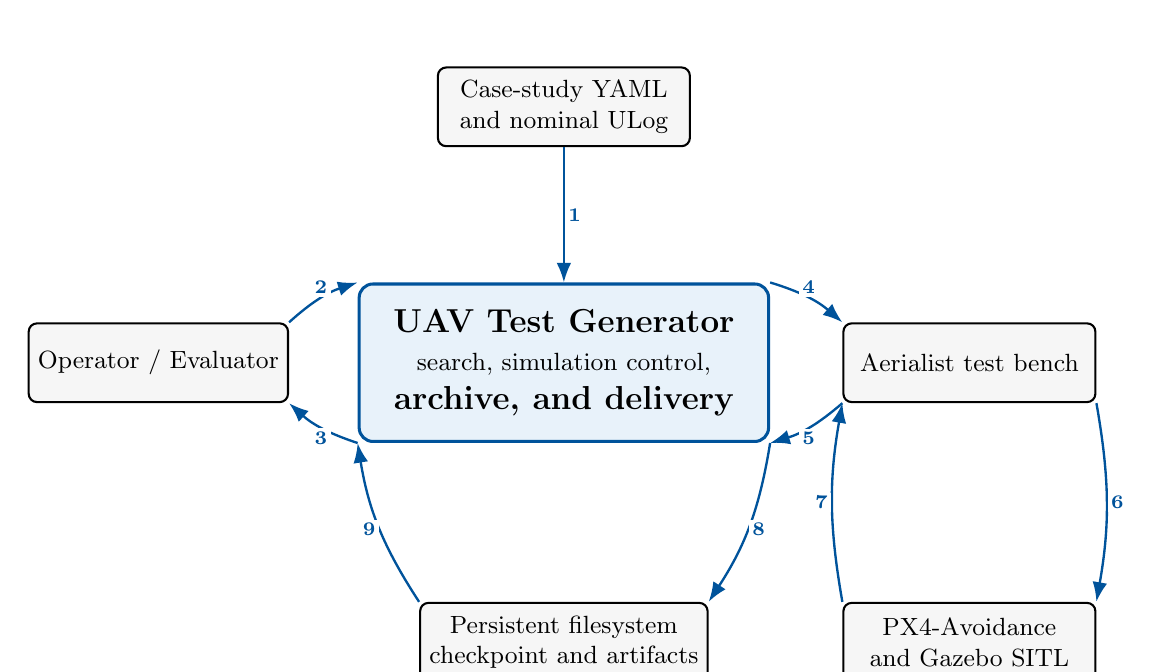
\begin{tikzpicture}[
  system/.style={
    draw=PolimiBlue,
    rounded corners=5pt,
    align=center,
    minimum width=5.2cm,
    minimum height=2.0cm,
    fill=LightBlue,
    line width=1.1pt,
    font=\large\bfseries
  },
  external/.style={
    draw,
    rounded corners=3pt,
    align=center,
    minimum width=3.2cm,
    minimum height=1.0cm,
    fill=LightGray,
    line width=0.75pt
  },
  flow/.style={-{Latex[length=2.5mm]}, line width=0.85pt, PolimiBlue},
  tag/.style={font=\scriptsize\bfseries, fill=white, inner sep=1.2pt},
  font=\small
]
\node[system] (system) at (0,0)
{UAV Test Generator\\
\normalfont\small search, simulation control,\\archive, and delivery};
\node[external] (mission) at (0,3.25)
{Case-study YAML\\and nominal ULog};
\node[external] (operator) at (-5.15,0)
{Operator / Evaluator};
\node[external] (aerialist) at (5.15,0)
{Aerialist test bench};
\node[external] (fs) at (0,-3.55)
{Persistent filesystem\\checkpoint and artifacts};
\node[external] (sim) at (5.15,-3.55)
{PX4-Avoidance\\and Gazebo SITL};

\draw[flow] (mission.south) -- node[tag,right]{1} (system.north);

\draw[flow] (operator.north east) to[bend left=12]
  node[tag,above,pos=0.50]{2} (system.north west);
\draw[flow] (system.south west) to[bend left=12]
  node[tag,below,pos=0.50]{3} (operator.south east);

\draw[flow] (system.north east) to[bend left=12]
  node[tag,above,pos=0.50]{4} (aerialist.north west);
\draw[flow] (aerialist.south west) to[bend left=12]
  node[tag,below,pos=0.50]{5} (system.south east);

\draw[flow] (aerialist.south east) to[bend left=10]
  node[tag,right,pos=0.50]{6} (sim.north east);
\draw[flow] (sim.north west) to[bend left=10]
  node[tag,left,pos=0.50]{7} (aerialist.south west);

\draw[flow] (system.south east) to[bend left=12]
  node[tag,right,pos=0.52]{8} (fs.north east);
\draw[flow] (fs.north west) to[bend left=12]
  node[tag,left,pos=0.48]{9} (system.south west);
\end{tikzpicture}

\vspace{0.25em}
\begin{minipage}{0.94\textwidth}
\footnotesize
\renewcommand{\arraystretch}{1.06}
\begin{tabularx}{\textwidth}{L{0.55cm} Y L{0.55cm} Y}
\textbf{1} & Mission definition and nominal route
& \textbf{2} & Mission, budget, and parameters\\
\textbf{3} & Progress and final delivery path
& \textbf{4} & Candidate test description\\
\textbf{5} & Trajectory and execution result
& \textbf{6} & Runtime execution request\\
\textbf{7} & Telemetry and flight log
& \textbf{8} & Checkpoint, YAML, ULog, plots, and ranks\\
\textbf{9} & Resume state and stored artifacts
& & \\
\end{tabularx}
\end{minipage}
\caption{System context and externally observable information flows. The generator is treated as a black box at requirements level.}
\label{fig:context}
\end{figure}

\section{Stakeholders and User Characteristics}
\begin{table}[H]
\centering
\begin{tabularx}{\textwidth}{L{3.2cm} Y Y}
\toprule
\textbf{Stakeholder} & \textbf{Interest} & \textbf{Relevant characteristics}\\
\midrule
Project developer & Correctness, maintainability, testability, and extensibility of the generator. & Familiar with Python, Docker, search-based testing, and the repository structure.\\
Competition evaluator & Automated execution, valid outputs, bounded resource use, and ordered failing tests. & Interacts through the prescribed command-line interface and generated files.\\
Experiment operator & Reproducible campaign execution, clear logs, crash recovery, and result inspection. & Comfortable with Linux shell commands and environment variables.\\
Course instructor / reviewer & Consistency among requirements, design, code, tests, and documented results. & Requires precise models, traceability, and technically justified choices.\\
UAV software engineer & Actionable failing scenarios and interpretable flight artifacts. & Understands UAV missions and flight logs but need not understand the search implementation.\\
\bottomrule
\end{tabularx}
\end{table}

\section{Operating Environment}
The reference environment is:
\begin{itemize}
  \item a Linux host with Docker support;
  \item the official Aerialist Docker image;
  \item Python 3 and the dependencies declared by the repository;
  \item a persistent host directory mounted into the container for code, checkpoints, logs, and generated tests;
  \item sufficient CPU, memory, and disk resources to execute PX4/Gazebo software-in-the-loop simulations.
\end{itemize}

The tool is command-line based and does not require a graphical interface. Simulations may run headlessly. A non-headless mode may be enabled for visual inspection when an X11 display is available.

\section{Assumptions and Dependencies}
\subsection{Assumptions}
\begin{enumerate}[label=\textbf{A-\arabic*:}]
  \item The supplied case-study YAML is syntactically valid and can be parsed by Aerialist.
  \item The mission, vehicle configuration, simulator, and required resources referenced by the case study are available to Aerialist.
  \item Aerialist returns at least one execution result containing a trajectory and a log file for successful simulations.
  \item The minimum distance computed by Aerialist is an adequate observable for detecting safety-distance violations.
  \item The persistent output directory remains available across container restarts.
  \item The host clock and filesystem support unique run-directory creation and atomic file replacement.
  \item Simulator non-determinism may cause repeated executions of the same test case to produce different trajectories and distances.
\end{enumerate}

\subsection{External Dependencies}
\begin{enumerate}[label=\textbf{D-\arabic*:}]
  \item Aerialist APIs for loading test descriptions, creating obstacles, executing tests, extracting trajectories, and serialising YAML.
  \item PX4-Avoidance and Gazebo for software-in-the-loop execution.
  \item NumPy for trajectory aggregation and numerical processing.
  \item Matplotlib for plot generation.
  \item PyYAML for reading obstacle definitions in plotting utilities.
  \item Shapely geometry operations provided through Aerialist obstacle objects.
  \item Docker for the reference deployment and crash-restart wrapper.
\end{enumerate}

\section{Competition and Domain Constraints}
\label{sec:constraints}
The following constraints are mandatory for generated test cases:
\begin{enumerate}[label=\textbf{C-\arabic*:}]
  \item A test case shall contain at least one and at most three box-shaped obstacles.
  \item Every obstacle shall be placed on the ground, with $z=0$.
  \item Obstacle dimensions and poses shall remain within the official ranges encoded by the project configuration:
  \[
  2 \le l \le 20,\quad 2 \le w \le 20,\quad 10 \le h \le 25,
  \]
  \[
  -40 \le x \le 30,\quad 10 \le y \le 40,\quad 0^\circ \le r \le 90^\circ.
  \]
  \item The complete rotated footprint of every obstacle shall fit inside the legal placement area; validity shall not be checked only at the obstacle centre.
  \item Obstacles in the same test case shall not overlap in the horizontal plane.
  \item The generator shall not modify the mission plan, UAV software configuration, or non-obstacle simulation properties of the input case study.
  \item The number of simulation attempts shall not exceed the declared budget. Retries, route bootstrapping, and confirmation runs consume budget.
  \item A single simulation shall be subject to a configurable timeout, whose reference value is $500\,\mathrm{s}$.
  \item The final delivery shall contain no more than the configured archive capacity, whose reference value is 20 tests.
\end{enumerate}

\section{Product Functions}
At a high level, the product shall:
\begin{enumerate}
  \item parse the command-line invocation and configure the selected generator;
  \item load the mission and obtain a nominal route if adaptive sampling is enabled;
  \item initialise or restore the search state;
  \item generate valid obstacle configurations;
  \item execute simulations while respecting budget and timeout constraints;
  \item compute failure severity, completion information, trajectory descriptors, and ranking data;
  \item evolve candidates through selection, mutation, step-size adaptation, and restart;
  \item persist all discovered failures and the resumable search state;
  \item construct a diverse, ordered final delivery suite;
  \item provide a random-search baseline with the same evaluation and output infrastructure.
\end{enumerate}

\section{Principal Scenarios}
\subsection{SC-01: Successful Evolutionary Campaign}
\textbf{Initial condition:} no checkpoint exists, the mission is valid, and the simulator is operational.

\textbf{Flow:}
\begin{enumerate}
  \item The operator invokes the generator with a mission and a budget.
  \item The system loads the mission and nominal route, or performs a route bootstrap when required.
  \item The system evaluates an initial set of candidates and selects the best as the parent.
  \item Until the budget is exhausted, the system mutates the parent, executes the child, updates the parent and mutation scale, archives failures, and checkpoints the state.
  \item The system selects trajectory-distinct failures, orders them by delivery score, copies their artifacts into the delivery directory, and reports its location.
\end{enumerate}

\subsection{SC-02: Simulator Failure and Automatic Recovery}
\textbf{Initial condition:} a candidate is marked as pending in the checkpoint and the simulator or container terminates unexpectedly.

\textbf{Flow:}
\begin{enumerate}
  \item The wrapper detects a non-zero container exit code.
  \item The wrapper starts a new container using the same persistent output directory.
  \item The generator loads the checkpoint, archive, parent, mutation scale, route, and pending genes.
  \item The interrupted candidate is re-executed from the beginning.
  \item Search continues until the global budget or restart limit is reached.
\end{enumerate}

\subsection{SC-03: Nominal Route Is Missing}
\textbf{Initial condition:} adaptive sampling is enabled, but no usable nominal ULog exists.

\textbf{Flow:}
\begin{enumerate}
  \item The system runs one simulation without generated obstacles.
  \item The resulting trajectory becomes the nominal route and its last point becomes the destination.
  \item The system tunes positional mutation scales to the route corridor.
  \item The route and destination are persisted in the checkpoint so that bootstrapping is not repeated after a crash.
\end{enumerate}

\subsection{SC-04: Critical Candidate Requires Confirmation}
\textbf{Initial condition:} a candidate produces an observed minimum distance below the configured confirmation threshold.

\textbf{Flow:}
\begin{enumerate}
  \item The system schedules the configured number of additional executions, provided budget remains.
  \item It aggregates the execution results, retains the most severe observed test artifact, computes the average competition point and execution time, and averages the resampled trajectories.
  \item The aggregate candidate is used by the archive and delivery logic.
\end{enumerate}

\subsection{SC-05: Redundant Failure}
\textbf{Initial condition:} a new failure has a trajectory within the configured DTW threshold of an archived failure.

\textbf{Flow:}
\begin{enumerate}
  \item The system permanently saves the new failure in the complete failure-history directory.
  \item If the new failure is more severe, it replaces the archived representative of the trajectory basin.
  \item Otherwise it is excluded from the delivery archive and contributes additional stagnation pressure.
\end{enumerate}

\subsection{SC-06: Random Baseline Campaign}
\textbf{Initial condition:} the generator mode is configured as random.

\textbf{Flow:}
\begin{enumerate}
  \item The system uses the same case loading, legal domain, simulation execution, budget accounting, failure archive, checkpoint, and delivery logic as the evolutionary generator.
  \item Every new candidate is sampled independently and does not depend on the parent, mutation scale, or targeted restart.
  \item The generated results can be compared with the evolutionary strategy without changing the evaluation infrastructure.
\end{enumerate}

\section{Domain Model}
\begin{figure}[H]
\centering
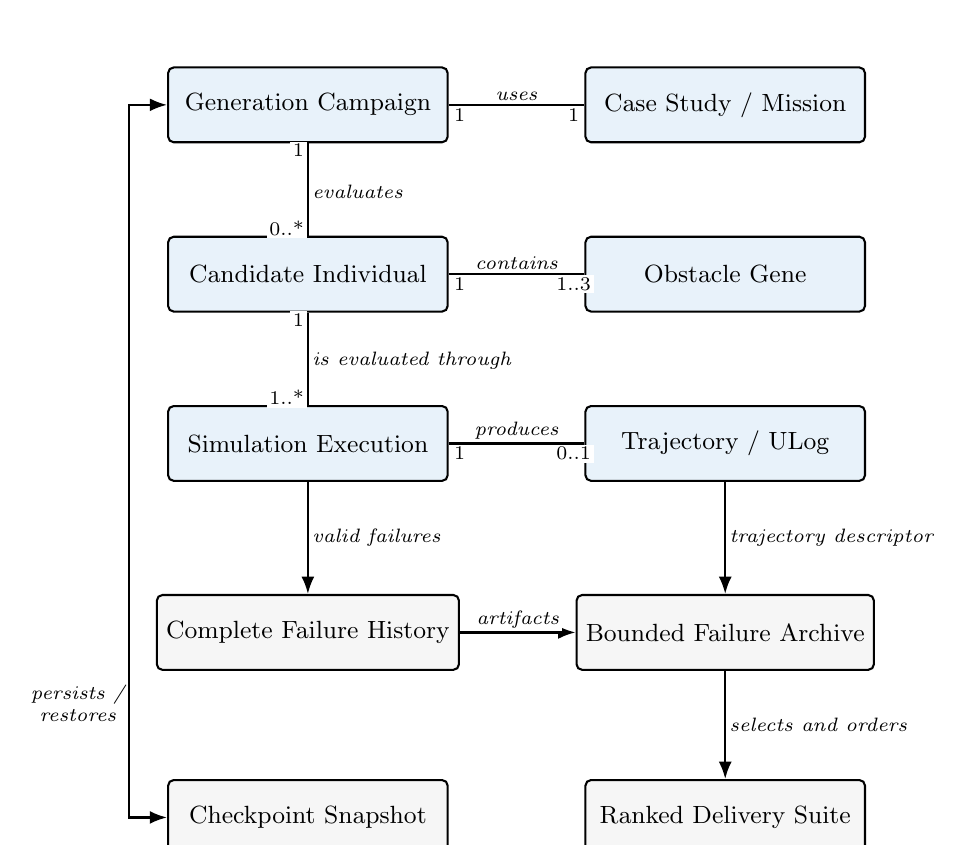
\begin{tikzpicture}[
  entity/.style={
    draw,
    rounded corners=2pt,
    fill=LightBlue,
    minimum width=3.55cm,
    minimum height=0.95cm,
    align=center,
    line width=0.75pt
  },
  store/.style={
    draw,
    rounded corners=2pt,
    fill=LightGray,
    minimum width=3.55cm,
    minimum height=0.95cm,
    align=center,
    line width=0.75pt
  },
  assoc/.style={line width=0.8pt},
  arrow/.style={-{Latex[length=2.2mm]}, line width=0.85pt},
  sync/.style={{Latex[length=2.2mm]}-{Latex[length=2.2mm]}, line width=0.85pt},
  mult/.style={font=\scriptsize, fill=white, inner sep=1pt},
  role/.style={font=\scriptsize\itshape, fill=white, inner sep=1.2pt, align=center},
  font=\small
]
\node[entity] (campaign) at (-2.65,0) {Generation Campaign};
\node[entity] (mission) at (2.65,0) {Case Study / Mission};

\node[entity] (candidate) at (-2.65,-2.15) {Candidate Individual};
\node[entity] (gene) at (2.65,-2.15) {Obstacle Gene};

\node[entity] (execution) at (-2.65,-4.30) {Simulation Execution};
\node[entity] (trajectory) at (2.65,-4.30) {Trajectory / ULog};

\node[store] (history) at (-2.65,-6.70) {Complete Failure History};
\node[store] (archive) at (2.65,-6.70) {Bounded Failure Archive};

\node[store] (checkpoint) at (-2.65,-9.05) {Checkpoint Snapshot};
\node[store] (delivery) at (2.65,-9.05) {Ranked Delivery Suite};

\draw[assoc] (campaign) -- node[role,above,pos=0.50]{uses} (mission)
  node[mult,below,pos=0.08]{1}
  node[mult,below,pos=0.92]{1};
\draw[assoc] (campaign) -- node[role,right,pos=0.52]{evaluates} (candidate)
  node[mult,left,pos=0.08]{1}
  node[mult,left,pos=0.92]{0..*};
\draw[assoc] (candidate) -- node[role,above,pos=0.50]{contains} (gene)
  node[mult,below,pos=0.08]{1}
  node[mult,below,pos=0.92]{1..3};
\draw[assoc] (candidate) -- node[role,right,pos=0.52]{is evaluated through} (execution)
  node[mult,left,pos=0.08]{1}
  node[mult,left,pos=0.92]{1..*};
\draw[assoc] (execution) -- node[role,above,pos=0.50]{produces} (trajectory)
  node[mult,below,pos=0.08]{1}
  node[mult,below,pos=0.92]{0..1};

\draw[arrow] (execution.south) --
  node[role,right]{valid failures}
  (history.north);
\draw[arrow] (trajectory.south) --
  node[role,right]{trajectory descriptor}
  (archive.north);
\draw[arrow] (history.east) --
  node[role,above]{artifacts}
  (archive.west);
\draw[arrow] (archive.south) --
  node[role,right]{selects and orders}
  (delivery.north);

\draw[sync] (campaign.west) -- ++(-0.48,0) |- 
  node[role,pos=0.42,left]{persists /\\restores}
  (checkpoint.west);
\end{tikzpicture}
\caption{Requirements-level domain model, separating durable evidence, bounded archive state, and final delivery.}
\label{fig:domain}
\end{figure}

\subsection{Domain Entities}
\begin{longtable}{L{3.2cm} L{11.5cm}}
\toprule
\textbf{Entity} & \textbf{Meaning and relevant information}\\
\midrule
\endfirsthead
\toprule
\textbf{Entity} & \textbf{Meaning and relevant information}\\
\midrule
\endhead
Generation Campaign & One invocation on one case study with one global budget, configuration, output directory, and selected generation method.\\
Case Study / Mission & Immutable Aerialist YAML input defining the UAV, mission, simulator, and environment to which generated obstacles are added.\\
Candidate Individual & Candidate scenario represented by genes and enriched after execution with fitness, minimum distance, completion state, average point, duration, trajectory, and file references.\\
Obstacle Gene & Six-dimensional tuple $[l,w,h,x,y,r]$ defining one box obstacle; $z$ is fixed to zero.\\
Simulation Execution & One budget-consuming attempt to run a candidate, possibly ending in success, timeout, execution failure, or process crash.\\
Trajectory / ULog & Recorded UAV motion used for distance measurement, mission-completion information, plotting, and behavioural diversity.\\
Failure Archive & Bounded set of representative failing individuals, one best representative per sufficiently distinct trajectory basin.\\
Delivery Suite & Ordered subset copied from persistent failures and intended for external evaluation.\\
Checkpoint & Atomic persistent snapshot of the search state and pending candidate.\\
\bottomrule
\end{longtable}

\section{Functional Requirements}
Each requirement is assigned a unique identifier and a priority. Mandatory requirements define the accepted product. ``Should'' requirements are important quality-enhancing functions implemented by the reference system. ``Could'' requirements are optional operational conveniences.

\subsection{Invocation and Configuration}
\begin{longtable}{L{1.7cm} L{2.1cm} L{10.8cm}}
\toprule
\textbf{ID} & \textbf{Priority} & \textbf{Requirement}\\
\midrule
\endfirsthead
\toprule
\textbf{ID} & \textbf{Priority} & \textbf{Requirement}\\
\midrule
\endhead
FR-01 & Mandatory & The system shall provide a command-line operation \texttt{generate <case-study> <budget>}.\\
FR-02 & Mandatory & The system shall reject or terminate unsuccessfully when the case-study path cannot be loaded, the budget is not an integer, or an unrecoverable initialisation error occurs.\\
FR-03 & Mandatory & The system shall support selecting the evolutionary generator or the random-search baseline without changing the command-line contract.\\
FR-04 & Mandatory & The system shall provide documented default values for all parameters required by an evaluator that supplies no optional environment variables.\\
FR-05 & Should & The system shall allow search, evaluation, timeout, archive, diversity, and reproducibility parameters to be overridden through environment variables.\\
\bottomrule
\end{longtable}

\subsection{Mission and Route Handling}
\begin{longtable}{L{1.7cm} L{2.1cm} L{10.8cm}}
\toprule
\textbf{ID} & \textbf{Priority} & \textbf{Requirement}\\
\midrule
\endfirsthead
\toprule
\textbf{ID} & \textbf{Priority} & \textbf{Requirement}\\
\midrule
\endhead
FR-06 & Mandatory & The system shall load the input case study through the Aerialist data model and preserve all input properties except the generated obstacle list.\\
FR-07 & Should & When adaptive sampling is enabled, the system shall attempt to extract a nominal $(x,y)$ route and destination from a corresponding ULog.\\
FR-08 & Should & If no nominal route is available, the system shall attempt one or more budget-accounted obstacle-free bootstrap simulations and use the recorded trajectory as the route.\\
FR-09 & Should & The system shall tune positional sampling or mutation scales to the extent of the obtained route while retaining the official legal bounds.\\
FR-10 & Mandatory & Failure to obtain a nominal route shall not make the generator unusable; the system shall fall back to a documented fixed sampling region.\\
\bottomrule
\end{longtable}

\subsection{Candidate Generation and Validity}
\begin{longtable}{L{1.7cm} L{2.1cm} L{10.8cm}}
\toprule
\textbf{ID} & \textbf{Priority} & \textbf{Requirement}\\
\midrule
\endfirsthead
\toprule
\textbf{ID} & \textbf{Priority} & \textbf{Requirement}\\
\midrule
\endhead
FR-11 & Mandatory & The system shall represent a candidate with one to three obstacle genes $[l,w,h,x,y,r]$.\\
FR-12 & Mandatory & Every generated obstacle shall satisfy the size, position, rotation, and ground-placement constraints defined in Section~\ref{sec:constraints}.\\
FR-13 & Mandatory & The system shall account for obstacle rotation when ensuring that the complete obstacle footprint fits within the legal area.\\
FR-14 & Mandatory & The system shall prevent or repair overlapping obstacles before simulation.\\
FR-15 & Mandatory & In evolutionary mode, the system shall generate each ordinary child by mutating the current parent and may add or remove an obstacle while preserving the allowed cardinality.\\
FR-16 & Should & When adding an obstacle to a candidate with a recorded trajectory, the system should be able to target an observed escape gap and orient the added obstacle across the local direction of motion.\\
FR-17 & Mandatory & In random mode, each ordinary candidate shall be sampled independently of previous candidates, the current parent, and the mutation scale.\\
\bottomrule
\end{longtable}

\subsection{Simulation and Measurement}
\begin{longtable}{L{1.7cm} L{2.1cm} L{10.8cm}}
\toprule
\textbf{ID} & \textbf{Priority} & \textbf{Requirement}\\
\midrule
\endfirsthead
\toprule
\textbf{ID} & \textbf{Priority} & \textbf{Requirement}\\
\midrule
\endhead
FR-18 & Mandatory & The system shall execute candidates through Aerialist using a copy of the original case study enriched with the generated obstacles.\\
FR-19 & Mandatory & Every simulation attempt, including retries, route bootstrap, and confirmation executions, shall increment the global budget counter exactly once.\\
FR-20 & Mandatory & The system shall not start a simulation attempt after the global budget has been exhausted.\\
FR-21 & Mandatory & The system shall enforce a configurable timeout for each simulation attempt and cancel the timeout after the attempt terminates.\\
FR-22 & Should & The system shall retry failed or timed-out simulation attempts up to a configurable limit while budget remains.\\
FR-23 & Mandatory & For every successful execution, the system shall compute the minimum distance between the trajectory and the generated obstacles.\\
FR-24 & Mandatory & The candidate fitness shall be the minimum observed distance; a lower value shall represent a better search result.\\
FR-25 & Should & The system shall determine whether the trajectory reaches a configurable neighbourhood of the nominal destination and record this information without using it to suppress a genuine safety violation.\\
FR-26 & Should & The system shall calculate the execution duration, competition point band, and a fixed-length resampled $(x,y)$ trajectory when sufficient log data are available.\\
FR-27 & Should & When the observed distance is below a configured criticality threshold, the system shall schedule additional confirmation executions, subject to the remaining budget, and aggregate the observations.\\
\bottomrule
\end{longtable}

\subsection{Evolutionary Search Control}
\begin{longtable}{L{1.7cm} L{2.1cm} L{10.8cm}}
\toprule
\textbf{ID} & \textbf{Priority} & \textbf{Requirement}\\
\midrule
\endfirsthead
\toprule
\textbf{ID} & \textbf{Priority} & \textbf{Requirement}\\
\midrule
\endhead
FR-28 & Mandatory & On a fresh evolutionary run, the system shall evaluate a configurable set of initial candidates and select the lowest-fitness candidate as the initial parent.\\
FR-29 & Mandatory & After each child evaluation, the system shall replace the parent if and only if the child has strictly lower fitness.\\
FR-30 & Mandatory & The system shall maintain an improvement history and adapt the mutation scale according to a documented success-rule policy within configured minimum and maximum limits.\\
FR-31 & Mandatory & The system shall maintain a stagnation counter and initiate a restart after a configured number of non-improving generations.\\
FR-32 & Should & A diversified restart should prefer a mission region insufficiently represented by the failure archive and should select among multiple candidates using geometric novelty.\\
FR-33 & Should & When the spatial regions are already covered, the system should probabilistically intensify the search around the most severe archived failure.\\
FR-34 & Should & A redundant failure should increase stagnation pressure so that the search leaves a behaviourally exhausted region earlier.\\
\bottomrule
\end{longtable}

\subsection{Failure Archive and Delivery}
\begin{longtable}{L{1.7cm} L{2.1cm} L{10.8cm}}
\toprule
\textbf{ID} & \textbf{Priority} & \textbf{Requirement}\\
\midrule
\endfirsthead
\toprule
\textbf{ID} & \textbf{Priority} & \textbf{Requirement}\\
\midrule
\endhead
FR-35 & Mandatory & A candidate with minimum distance below $1.5\,\mathrm{m}$ shall be treated as a valid failure independently of whether the destination was reached.\\
FR-36 & Mandatory & Every valid failure with available execution artifacts shall be persisted immediately in a complete failure-history directory before the next candidate is evaluated.\\
FR-37 & Mandatory & The persisted failure artifacts shall include the generated YAML and, when available, the corresponding ULog and official-style plot.\\
FR-38 & Mandatory & The system shall maintain a bounded delivery archive and shall identify behaviourally redundant failures using trajectory distance when trajectory data are available.\\
FR-39 & Mandatory & If a new failure belongs to the same trajectory basin as an archived failure, the system shall retain the one with the lower minimum distance as the archive representative.\\
FR-40 & Mandatory & When the archive is full, a new distinct failure shall enter only if it improves the archive according to the documented delivery-ranking criterion.\\
FR-41 & Mandatory & The final delivery shall contain an ordered subset whose retained trajectories satisfy the configured separation rule whenever trajectory data are available.\\
FR-42 & Mandatory & The delivery order shall be descending in the score
\[
S(t)=\frac{10\,\overline{p}(t)}{n_{\mathrm{obs}}(t)^2\,\overline{T}(t)},
\]
where $\overline{p}$ is the average point, $n_{\mathrm{obs}}$ is the number of obstacles, and $\overline{T}$ is the average execution time in minutes.\\
FR-43 & Mandatory & The final directory shall use stable rank-prefixed basenames such that \texttt{rank01} denotes the highest-ranked delivered test.\\
FR-44 & Mandatory & Rebuilding the final selection shall be idempotent and shall not delete the complete failure history.\\
\bottomrule
\end{longtable}

\subsection{Checkpointing, Recovery, and Logging}
\begin{longtable}{L{1.7cm} L{2.1cm} L{10.8cm}}
\toprule
\textbf{ID} & \textbf{Priority} & \textbf{Requirement}\\
\midrule
\endfirsthead
\toprule
\textbf{ID} & \textbf{Priority} & \textbf{Requirement}\\
\midrule
\endhead
FR-45 & Mandatory & The system shall save a checkpoint before executing a candidate and after completing each initial seed or generation.\\
FR-46 & Mandatory & Checkpoint creation shall use an atomic replacement strategy so that interruption during writing does not replace the last valid checkpoint with a partial file.\\
FR-47 & Mandatory & A checkpoint shall contain sufficient serialisable data to restore the budget counter, search parameters, parent, archive, pending candidate, initialisation state, nominal route, and destination.\\
FR-48 & Mandatory & On restart, the system shall restore a valid checkpoint from the same output directory and continue the campaign without resetting the global budget or archive.\\
FR-49 & Mandatory & A candidate marked as pending at the time of failure shall be executed again from the beginning using the same genes.\\
FR-50 & Should & The reference launcher should restart a failed container automatically up to a configurable limit and preserve host ownership of generated artifacts.\\
FR-51 & Mandatory & The system shall record detailed diagnostics in a persistent debug log and concise progress information on standard output.\\
FR-52 & Mandatory & At successful termination, the system shall report the final delivery-directory location and the number of delivered tests.\\
\bottomrule
\end{longtable}

\subsection{Visualisation and Inspection}
\begin{longtable}{L{1.7cm} L{2.1cm} L{10.8cm}}
\toprule
\textbf{ID} & \textbf{Priority} & \textbf{Requirement}\\
\midrule
\endfirsthead
\toprule
\textbf{ID} & \textbf{Priority} & \textbf{Requirement}\\
\midrule
\endhead
FR-53 & Should & For each persisted failure with a readable ULog, the system should generate a plot containing $x$, $y$, $z$, and yaw versus time and a top-down trajectory view with rotated obstacle footprints.\\
FR-54 & Should & Plot-generation failure shall be logged but shall not terminate the search or invalidate otherwise usable YAML and ULog artifacts.\\
FR-55 & Could & The launcher may support a non-headless simulation mode for interactive debugging while retaining headless execution as the default.\\
\bottomrule
\end{longtable}

\section{Data Requirements}
\subsection{Input Data}
The minimum input is a case-study path and a simulation budget. Optional configuration is supplied through environment variables. The case study is interpreted by Aerialist and must contain the information necessary to instantiate the UAV, simulator, mission, and initial environment.

\subsection{Persistent Output Data}
A generation campaign shall produce a self-contained output tree containing, as applicable:
\begin{itemize}
  \item a persistent debug log;
  \item an atomic JSON checkpoint;
  \item a complete failure-history directory containing YAML, ULog, and plot artifacts;
  \item a delivery directory containing ordered rank-prefixed copies;
  \item any launcher or simulator diagnostics required to analyse failures.
\end{itemize}

\subsection{Checkpoint Integrity}
Only JSON-safe values shall be persisted. External Aerialist objects shall not be serialised directly. Values representing unavailable infinity shall be encoded using an explicit nullable representation. Persistent references to failure artifacts shall be relative to the campaign output directory to preserve relocatability.

\section{Non-Functional Requirements}
\begin{longtable}{L{1.7cm} L{3.0cm} L{9.9cm}}
\toprule
\textbf{ID} & \textbf{Category} & \textbf{Requirement}\\
\midrule
\endfirsthead
\toprule
\textbf{ID} & \textbf{Category} & \textbf{Requirement}\\
\midrule
\endhead
NFR-01 & Correctness & The generator shall enforce the obstacle cardinality, legal-domain, ground-placement, and non-overlap constraints before executing a candidate.\\
NFR-02 & Budget safety & The recorded number of attempts shall never exceed the declared simulation budget.\\
NFR-03 & Recoverability & After an unexpected termination, all failures persisted before the termination and the latest valid checkpoint shall remain usable.\\
NFR-04 & Reliability & A timeout, failed simulation, missing optional plot dependency, or unreadable optional nominal log shall be handled without corrupting persistent state.\\
NFR-05 & Reproducibility & Supplying the same explicit pseudo-random seed and configuration shall reproduce the generator's sampling and mutation decisions, although simulator outputs may remain non-deterministic.\\
NFR-06 & Performance & Trajectory comparison shall operate on a bounded resampled representation rather than unbounded raw logs, and archive size shall remain bounded.\\
NFR-07 & Portability & The reference deployment shall run in Docker on a Linux host without requiring installation of PX4/Gazebo directly on the host.\\
NFR-08 & Maintainability & Search configuration, geometry and scoring, data model, orchestration, execution wrapper, plotting, and CLI concerns shall be separated into identifiable modules.\\
NFR-09 & Extensibility & A baseline generator shall reuse common execution and delivery infrastructure while replacing the candidate-generation policy through subclassing or an equivalent variation mechanism.\\
NFR-10 & Observability & Logs shall expose mission, budget progress, generated obstacle parameters, measured distance, completion information, restart events, archive decisions, and final delivery information.\\
NFR-11 & Usability & A standard campaign shall be startable through one documented shell command and shall print the output location at termination.\\
NFR-12 & Traceability & Every mandatory functional requirement shall map to one or more design components and implementation modules in the Design Document.\\
NFR-13 & Data preservation & Constructing or reconstructing the delivery suite shall never remove the complete failure-history artifacts.\\
NFR-14 & Graceful degradation & Missing trajectory, flight-duration, or optional plotting data shall trigger documented fallback behaviour rather than an unhandled exception.\\
NFR-15 & Testability & Pure geometry, scoring, serialisation, archive, and selection behaviour shall be separable from expensive simulator execution so that automated tests can exercise deterministic logic.\\
\bottomrule
\end{longtable}

\section{Excluded Requirements}
The following capabilities are explicitly outside the project scope:
\begin{itemize}
  \item modification or verification of the internal PX4-Avoidance source code;
  \item formal proof of collision avoidance or simulator fidelity;
  \item real-world UAV flight execution;
  \item optimisation of wind, lighting, sensor noise, or non-box obstacle types;
  \item a graphical campaign-management application;
  \item distributed Kubernetes scheduling implemented by the generator itself;
  \item permanent deletion of generated failures or automatic upload to an external evaluator.
\end{itemize}

% ===========================================================================
\chapter{Additional Models}
% ===========================================================================

\section{Use-Case Model}
\begin{figure}[H]
\centering
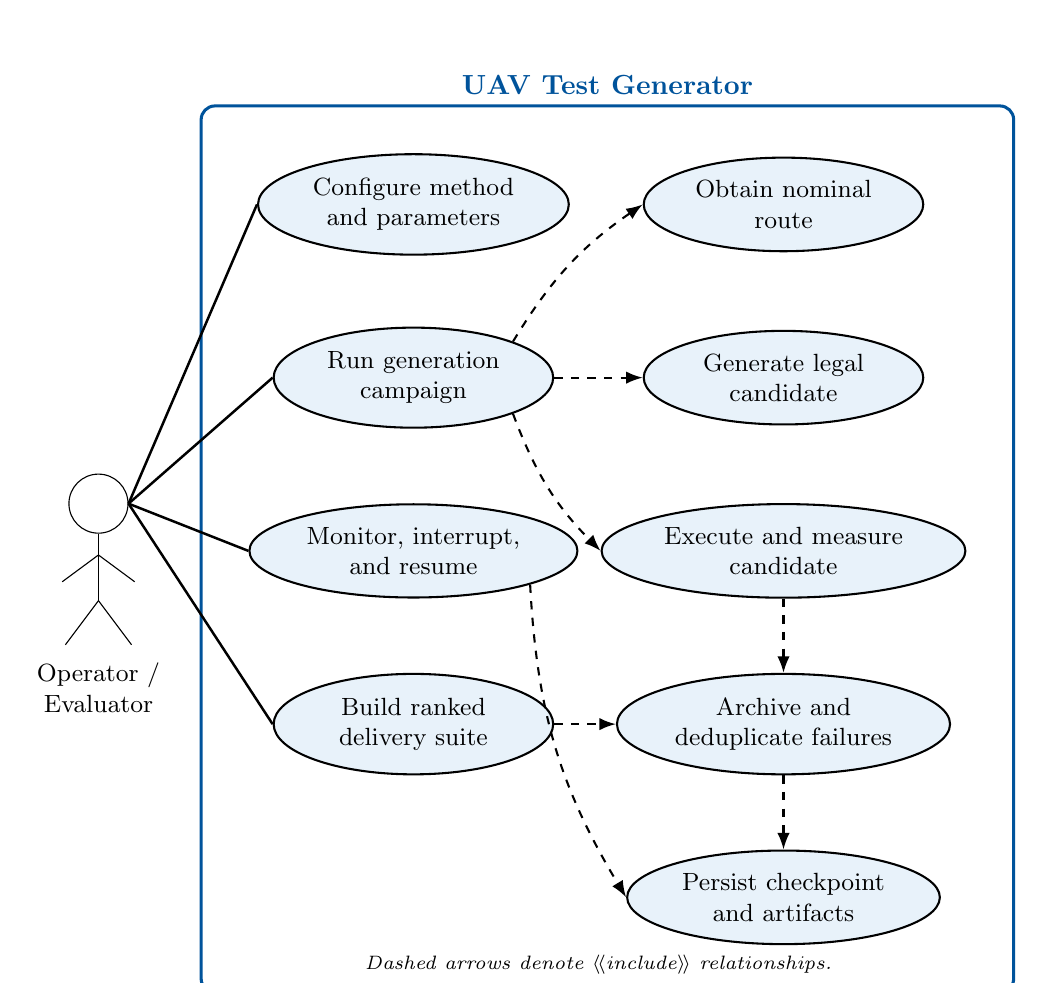
\begin{tikzpicture}[
  usecase/.style={
    draw,
    ellipse,
    align=center,
    minimum width=3.55cm,
    minimum height=1.0cm,
    fill=LightBlue,
    line width=0.75pt,
    font=\small
  },
  assoc/.style={line width=0.9pt},
  include/.style={-{Latex[length=2.1mm]}, dashed, line width=0.75pt},
  ilabel/.style={font=\scriptsize, fill=white, inner sep=1.2pt},
  font=\small
]
% Actor
\node[draw,circle,minimum size=7.5mm,inner sep=0pt] (head) at (-5.3,0.2) {};
\draw (head.south) -- ++(0,-0.85);
\draw ($(head.south)+(0,-0.27)$) -- ++(-0.46,-0.34);
\draw ($(head.south)+(0,-0.27)$) -- ++(0.46,-0.34);
\draw ($(head.south)+(0,-0.85)$) -- ++(-0.42,-0.56);
\draw ($(head.south)+(0,-0.85)$) -- ++(0.42,-0.56);
\node[below=1.52cm of head,font=\small,align=center] {Operator /\\Evaluator};

% User-facing use cases
\node[usecase] (configure) at (-1.3,4.0) {Configure method\\and parameters};
\node[usecase] (run)       at (-1.3,1.8) {Run generation\\campaign};
\node[usecase] (monitor)   at (-1.3,-0.4) {Monitor, interrupt,\\and resume};
\node[usecase] (delivery)  at (-1.3,-2.6) {Build ranked\\delivery suite};

% Campaign services
\node[usecase] (route)     at (3.4,4.0) {Obtain nominal\\route};
\node[usecase] (candidate) at (3.4,1.8) {Generate legal\\candidate};
\node[usecase] (execute)   at (3.4,-0.4) {Execute and measure\\candidate};
\node[usecase] (archive)   at (3.4,-2.6) {Archive and\\deduplicate failures};
\node[usecase] (persist)   at (3.4,-4.8) {Persist checkpoint\\and artifacts};

\begin{scope}[on background layer]
\node[
  draw=PolimiBlue,
  fill=none,
  rounded corners=5pt,
  line width=1.1pt,
  fit=(configure)(run)(monitor)(delivery)(route)(candidate)(execute)(archive)(persist),
  inner sep=6mm,
  label={[PolimiBlue,font=\bfseries]above:UAV Test Generator}
] {};
\end{scope}

\draw[assoc] (head.east) -- (configure.west);
\draw[assoc] (head.east) -- (run.west);
\draw[assoc] (head.east) -- (monitor.west);
\draw[assoc] (head.east) -- (delivery.west);

\draw[include] (run.north east) to[bend left=12]
  (route.west);
\draw[include] (run.east) --
  (candidate.west);
\draw[include] (run.south east) to[bend right=12]
  (execute.west);
\draw[include] (execute.south) --
  (archive.north);
\draw[include] (archive.south) --
  (persist.north);
\draw[include] (delivery.east) --
  (archive.west);
\draw[include] (monitor.south east) to[bend right=14]
  (persist.west);
\node[font=\scriptsize\itshape,align=center] at (1.05,-5.65)
{Dashed arrows denote $\langle\!\langle$include$\rangle\!\rangle$ relationships.};
\end{tikzpicture}
\caption{Primary evaluator-facing use cases and the campaign services they include.}
\label{fig:usecases}
\end{figure}

\subsection{UC-01: Run Generation Campaign}
\begin{tabularx}{\textwidth}{L{3.4cm} Y}
\toprule
Primary actor & Operator or competition evaluator\\
Preconditions & Valid execution environment; readable case-study path; positive integer budget\\
Trigger & Invocation of the \texttt{generate} command\\
Main success result & Budget-bounded campaign completes and an ordered delivery directory is produced\\
Failure result & Process exits non-zero with persistent diagnostics; previously saved state remains available\\
Related requirements & FR-01--FR-05, FR-18--FR-24, FR-28--FR-52\\
\bottomrule
\end{tabularx}

\subsection{UC-02: Resume Interrupted Campaign}
\begin{tabularx}{\textwidth}{L{3.4cm} Y}
\toprule
Primary actor & Launcher / operator\\
Preconditions & Persistent output directory contains a valid checkpoint\\
Trigger & Process or container restarts after an unexpected termination\\
Main success result & Search state is restored and the pending candidate is re-executed without resetting the archive or budget\\
Alternative result & If the checkpoint is unreadable, the system reports the condition and performs the documented clean-start behaviour\\
Related requirements & FR-45--FR-51; NFR-03, NFR-04, NFR-13\\
\bottomrule
\end{tabularx}

\subsection{UC-03: Construct Final Delivery}
\begin{tabularx}{\textwidth}{L{3.4cm} Y}
\toprule
Primary actor & Competition evaluator\\
Preconditions & The campaign has an archive and/or persistent failure artifacts\\
Trigger & Search budget is exhausted or final selection is explicitly rebuilt\\
Main success result & A rank-ordered, diversity-filtered suite is copied into the delivery directory\\
Postconditions & Complete failure history is unchanged; obsolete rank copies may be removed only from the delivery directory\\
Related requirements & FR-35--FR-44, FR-52; NFR-13\\
\bottomrule
\end{tabularx}

\section{Requirements-Level Sequence Model}
\begin{figure}[H]
\centering
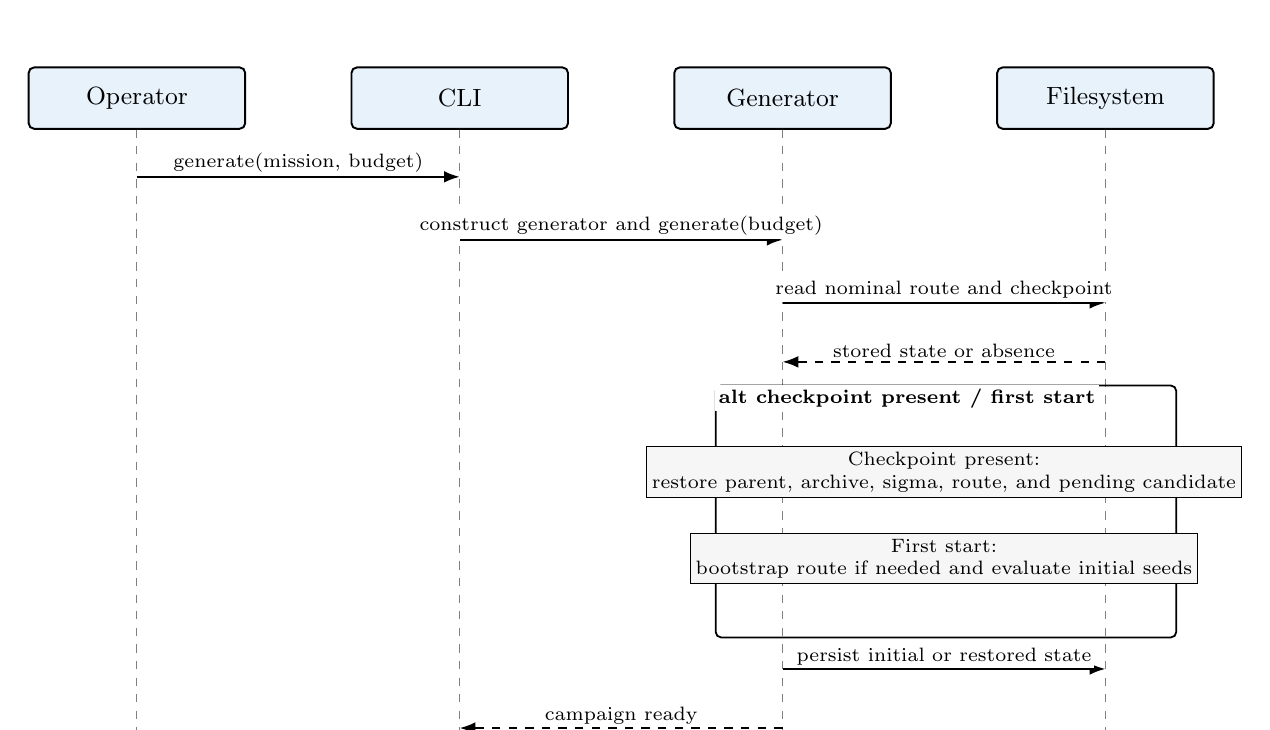
\begin{tikzpicture}[
  participant/.style={
    draw,
    rounded corners=2pt,
    fill=LightBlue,
    minimum width=2.75cm,
    minimum height=0.78cm,
    align=center,
    line width=0.7pt
  },
  msg/.style={-{Latex[length=2mm]}, line width=0.75pt},
  ret/.style={-{Latex[length=2mm]}, dashed, line width=0.65pt},
  frame/.style={draw, rounded corners=2pt, line width=0.65pt},
  framelabel/.style={anchor=north west, font=\scriptsize\bfseries, fill=white, inner sep=1.2pt},
  note/.style={draw, fill=LightGray, align=center, font=\scriptsize, inner sep=2pt},
  textlabel/.style={font=\scriptsize, fill=white, inner sep=1.1pt},
  font=\small
]
\def\XUser{0}
\def\XCLI{4.1}
\def\XGen{8.2}
\def\XFS{12.3}
\node[participant] (user) at (\XUser,0) {Operator};
\node[participant] (cli) at (\XCLI,0) {CLI};
\node[participant] (gen) at (\XGen,0) {Generator};
\node[participant] (fs) at (\XFS,0) {Filesystem};
\foreach \x in {\XUser,\XCLI,\XGen,\XFS}
  \draw[dashed,gray] (\x,-0.40) -- (\x,-8.15);

\draw[msg] (\XUser,-1.0) --
  node[textlabel,above]{generate(mission, budget)}
  (\XCLI,-1.0);
\draw[msg] (\XCLI,-1.8) --
  node[textlabel,above]{construct generator and generate(budget)}
  (\XGen,-1.8);
\draw[msg] (\XGen,-2.6) --
  node[textlabel,above]{read nominal route and checkpoint}
  (\XFS,-2.6);
\draw[ret] (\XFS,-3.35) --
  node[textlabel,above]{stored state or absence}
  (\XGen,-3.35);

\node[frame,fit={(7.55,-3.85) (13.0,-6.65)},inner sep=2mm] (initframe) {};
\node[framelabel] at (initframe.north west) {alt checkpoint present / first start};
\node[note] at (10.25,-4.75)
{Checkpoint present:\\restore parent, archive, sigma, route, and pending candidate};
\node[note] at (10.25,-5.85)
{First start:\\bootstrap route if needed and evaluate initial seeds};

\draw[msg] (\XGen,-7.25) --
  node[textlabel,above]{persist initial or restored state}
  (\XFS,-7.25);
\draw[ret] (\XGen,-8.0) --
  node[textlabel,above]{campaign ready}
  (\XCLI,-8.0);
\end{tikzpicture}
\caption{Requirements-level interaction for campaign invocation, initialisation, and recovery.}
\label{fig:reqsequence-init}
\end{figure}

\begin{figure}[H]
\centering
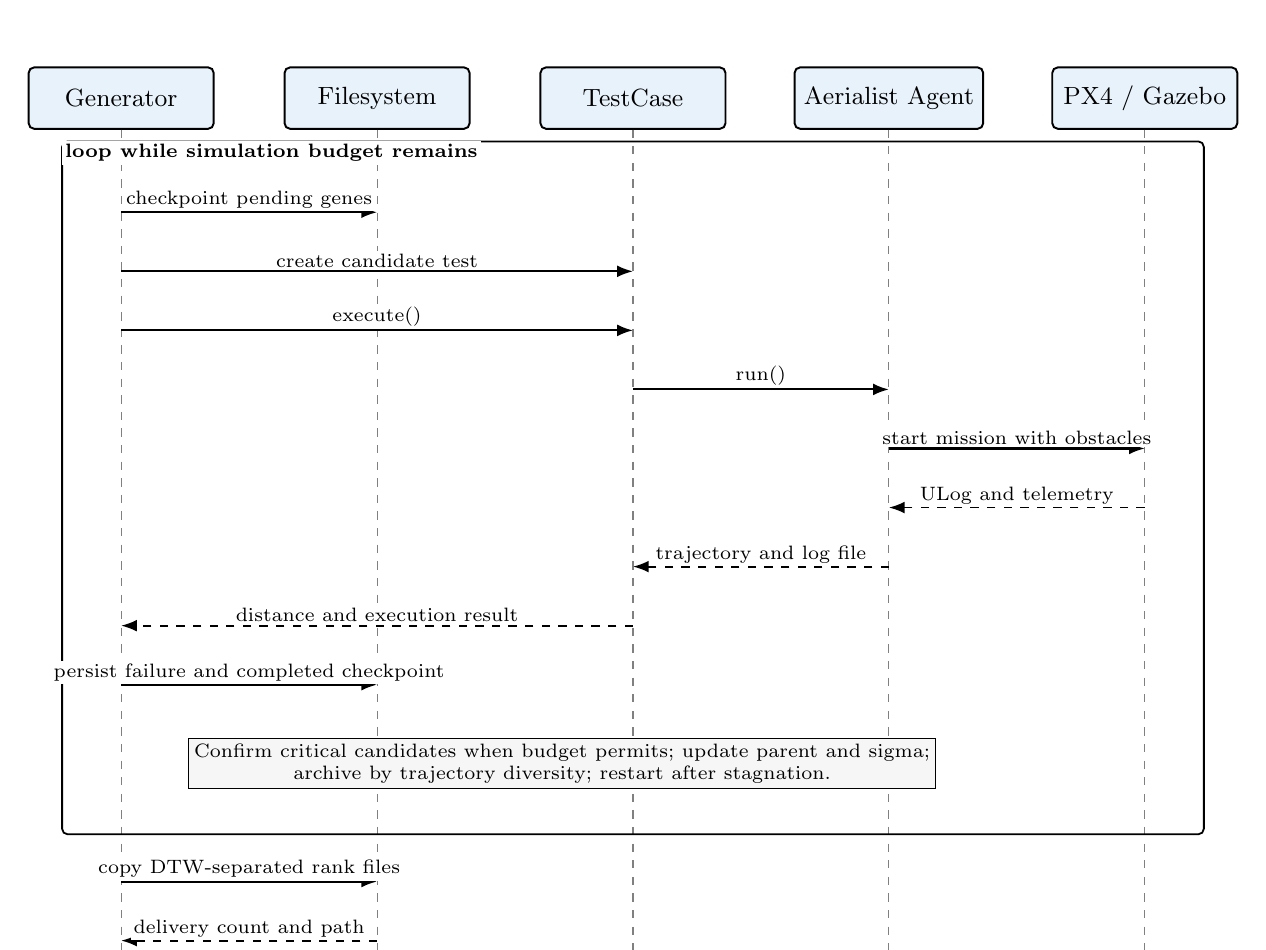
\begin{tikzpicture}[
  participant/.style={
    draw,
    rounded corners=2pt,
    fill=LightBlue,
    minimum width=2.35cm,
    minimum height=0.78cm,
    align=center,
    line width=0.7pt
  },
  msg/.style={-{Latex[length=2mm]}, line width=0.75pt},
  ret/.style={-{Latex[length=2mm]}, dashed, line width=0.65pt},
  frame/.style={draw, rounded corners=2pt, line width=0.65pt},
  framelabel/.style={anchor=north west, font=\scriptsize\bfseries, fill=white, inner sep=1.2pt},
  note/.style={draw, fill=LightGray, align=center, font=\scriptsize, inner sep=2pt},
  textlabel/.style={font=\scriptsize, fill=white, inner sep=1.0pt, align=center},
  font=\small
]
\def\XGen{0}
\def\XFS{3.25}
\def\XTC{6.50}
\def\XAgent{9.75}
\def\XSim{13.0}
\node[participant] (gen) at (\XGen,0) {Generator};
\node[participant] (fs) at (\XFS,0) {Filesystem};
\node[participant] (tc) at (\XTC,0) {TestCase};
\node[participant] (agent) at (\XAgent,0) {Aerialist Agent};
\node[participant] (sim) at (\XSim,0) {PX4 / Gazebo};
\foreach \x in {\XGen,\XFS,\XTC,\XAgent,\XSim}
  \draw[dashed,gray] (\x,-0.40) -- (\x,-10.95);

\node[frame,fit={(-0.55,-0.75) (13.55,-9.15)},inner sep=2mm] (loopframe) {};
\node[framelabel] at (loopframe.north west) {loop while simulation budget remains};
\draw[msg] (\XGen,-1.45) --
  node[textlabel,above]{checkpoint pending genes}
  (\XFS,-1.45);
\draw[msg] (\XGen,-2.20) --
  node[textlabel,above]{create candidate test}
  (\XTC,-2.20);
\draw[msg] (\XGen,-2.95) --
  node[textlabel,above]{execute()}
  (\XTC,-2.95);
\draw[msg] (\XTC,-3.70) --
  node[textlabel,above]{run()}
  (\XAgent,-3.70);
\draw[msg] (\XAgent,-4.45) --
  node[textlabel,above]{start mission with obstacles}
  (\XSim,-4.45);
\draw[ret] (\XSim,-5.20) --
  node[textlabel,above]{ULog and telemetry}
  (\XAgent,-5.20);
\draw[ret] (\XAgent,-5.95) --
  node[textlabel,above]{trajectory and log file}
  (\XTC,-5.95);
\draw[ret] (\XTC,-6.70) --
  node[textlabel,above]{distance and execution result}
  (\XGen,-6.70);
\draw[msg] (\XGen,-7.45) --
  node[textlabel,above]{persist failure and completed checkpoint}
  (\XFS,-7.45);
\node[note] at (5.6,-8.45)
{Confirm critical candidates when budget permits; update parent and sigma;\\
archive by trajectory diversity; restart after stagnation.};

\draw[msg] (\XGen,-9.95) --
  node[textlabel,above]{copy DTW-separated rank files}
  (\XFS,-9.95);
\draw[ret] (\XFS,-10.70) --
  node[textlabel,above]{delivery count and path}
  (\XGen,-10.70);
\end{tikzpicture}
\caption{Requirements-level interaction for candidate execution, archive update, checkpointing, and final delivery.}
\label{fig:reqsequence}
\end{figure}

\section{Campaign State Model}
\begin{figure}[H]
\centering
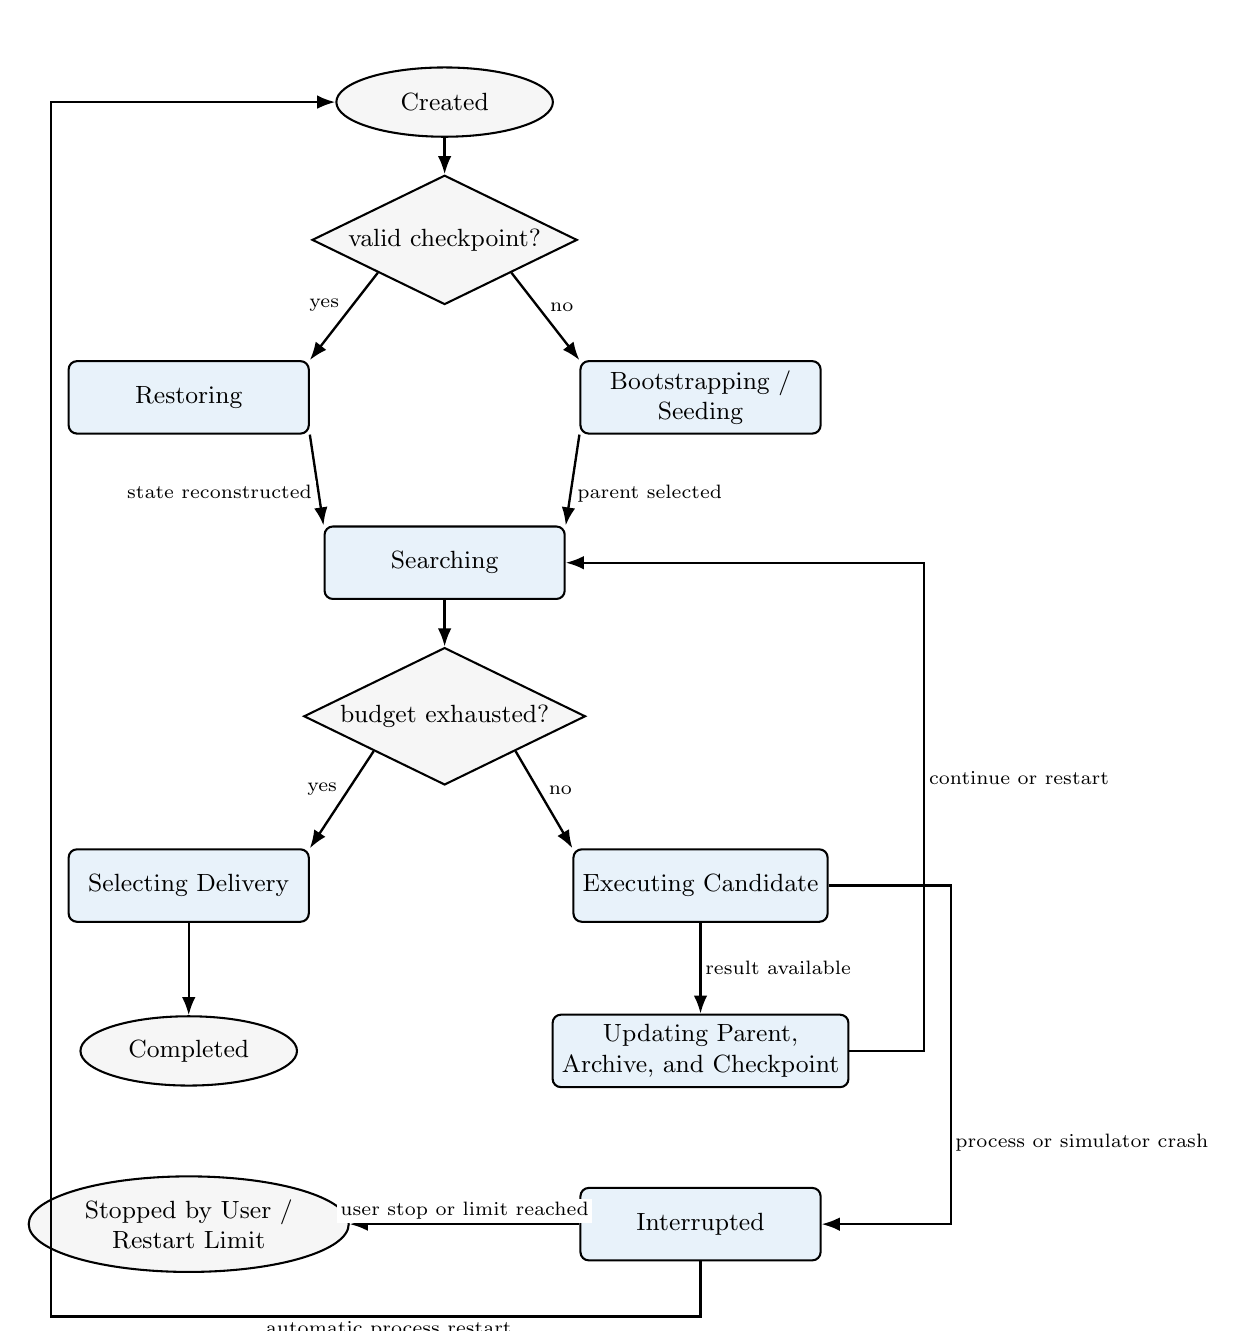
\begin{tikzpicture}[
  state/.style={
    draw,
    rounded corners=3pt,
    minimum width=3.05cm,
    minimum height=0.92cm,
    align=center,
    fill=LightBlue,
    line width=0.75pt
  },
  decision/.style={
    draw,
    diamond,
    aspect=2.05,
    align=center,
    fill=LightGray,
    line width=0.75pt,
    inner sep=1.6pt
  },
  terminal/.style={
    draw,
    ellipse,
    minimum width=2.75cm,
    minimum height=0.88cm,
    align=center,
    fill=LightGray,
    line width=0.75pt
  },
  arr/.style={-{Latex[length=2.3mm]}, line width=0.85pt},
  lab/.style={fill=white,inner sep=1.3pt,font=\scriptsize,align=center},
  font=\small
]
\node[terminal] (created) at (0,6.4) {Created};
\node[decision] (ckpt) at (0,4.65) {valid checkpoint?};
\node[state] (restore) at (-3.25,2.65) {Restoring};
\node[state] (seed) at (3.25,2.65) {Bootstrapping /\\Seeding};
\node[state] (search) at (0,0.55) {Searching};
\node[decision] (budget) at (0,-1.40) {budget exhausted?};

\node[state] (delivery) at (-3.25,-3.55) {Selecting Delivery};
\node[terminal] (complete) at (-3.25,-5.65) {Completed};
\node[state] (execute) at (3.25,-3.55) {Executing Candidate};
\node[state] (update) at (3.25,-5.65) {Updating Parent,\\Archive, and Checkpoint};
\node[state] (interrupted) at (3.25,-7.85) {Interrupted};
\node[terminal] (stopped) at (-3.25,-7.85) {Stopped by User /\\Restart Limit};

\draw[arr] (created) -- (ckpt);
\draw[arr] (ckpt.south west) --
  node[lab,above left]{yes}
  (restore.north east);
\draw[arr] (ckpt.south east) --
  node[lab,above right]{no}
  (seed.north west);
\draw[arr] (restore.south east) --
  node[lab,below left]{state reconstructed}
  (search.north west);
\draw[arr] (seed.south west) --
  node[lab,below right]{parent selected}
  (search.north east);
\draw[arr] (search) -- (budget);

\draw[arr] (budget.south west) --
  node[lab,above left]{yes}
  (delivery.north east);
\draw[arr] (delivery) -- (complete);
\draw[arr] (budget.south east) --
  node[lab,above right]{no}
  (execute.north west);
\draw[arr] (execute) --
  node[lab,right]{result available}
  (update);

\draw[arr] (update.east) -- ++(0.95,0) |- 
  node[lab,pos=0.28,right]{continue or restart}
  (search.east);
\draw[arr] (execute.east) -- ++(1.55,0) |- 
  node[lab,pos=0.38,right]{process or simulator crash}
  (interrupted.east);
\draw[arr] (interrupted.south) -- ++(0,-0.70) -| 
  node[lab,pos=0.24,below]{automatic process restart}
  (-5.0,6.4) -- (created.west);
\draw[arr] (interrupted.west) --
  node[lab,above]{user stop or limit reached}
  (stopped.east);
\end{tikzpicture}
\caption{Campaign lifecycle and crash-recovery transitions.}
\label{fig:statemodel}
\end{figure}

\begin{table}[H]
\centering
\begingroup
\small
\renewcommand{\arraystretch}{1.06}
\begin{tabularx}{\textwidth}{L{4.1cm} L{4.1cm} Y}
\toprule
\textbf{Source state} & \textbf{Target state} & \textbf{Trigger}\\
\midrule
Searching & Executing candidate & A candidate is ready and budget remains.\\
Executing candidate & Searching & The attempt terminates and state updates complete.\\
Searching & Selecting delivery & The global budget is exhausted.\\
Executing candidate & Interrupted & The process or simulator terminates unexpectedly.\\
Interrupted & Created & The launcher permits another process restart; the new process then validates and restores the checkpoint.\\
Interrupted & Stopped / failed & The restart limit is reached or the operator stops the run.\\
\bottomrule
\end{tabularx}
\endgroup
\end{table}

\section{Acceptance Criteria}
The product is acceptable when all of the following conditions hold:
\begingroup
\small
\begin{enumerate}[itemsep=1pt,topsep=3pt]
  \item The documented command runs on the reference Docker environment and accepts a mission YAML and budget.
  \item Automated tests confirm the legal obstacle domain, rotation-aware fitting, overlap rejection or repair, serialisation round-trip, scoring formulas, archive decisions, and final selection logic.
  \item A campaign cannot consume more simulation attempts than its declared budget.
  \item At least one deliberately interrupted campaign resumes from its checkpoint without losing already persisted failures.
  \item Every delivered YAML contains one to three legal non-overlapping obstacles and is accompanied by available ULog and plot artifacts.
  \item Delivery ranks are ordered by the documented score and rebuilding the delivery does not alter the complete failure-history directory.
  \item The evolutionary and random generators can be invoked through the same external interface and generate separate campaign outputs.
  \item The repository documentation identifies installation prerequisites, execution commands, parameter defaults, output structure, and authorship.
\end{enumerate}
\endgroup

\section{Scenario-to-Requirement Traceability}
\begingroup
\small
\renewcommand{\arraystretch}{1.03}
\begin{longtable}{L{2cm} L{12.8cm}}
\toprule
\textbf{Scenario} & \textbf{Principal requirements}\\
\midrule
\endfirsthead
\toprule
\textbf{Scenario} & \textbf{Principal requirements}\\
\midrule
\endhead
SC-01 & FR-01, FR-06, FR-11--FR-24, FR-28--FR-46, FR-51--FR-54; NFR-01, NFR-02, NFR-08, NFR-11\\
SC-02 & FR-19, FR-45--FR-51; NFR-03, NFR-04, NFR-13\\
SC-03 & FR-07--FR-10, FR-19, FR-47--FR-49; NFR-04, NFR-14\\
SC-04 & FR-19, FR-20, FR-23--FR-27, FR-35--FR-40; NFR-02, NFR-05\\
SC-05 & FR-34--FR-41, FR-44; NFR-06, NFR-13\\
SC-06 & FR-03, FR-17--FR-27, FR-35--FR-52; NFR-09\\
\bottomrule
\end{longtable}
\endgroup

% ===========================================================================
\chapter{References}
\label{chap:references}
% ===========================================================================

\begin{enumerate}[label={[\arabic*]},leftmargin=2.2em,itemsep=0.65em,topsep=0.4em]
\item M. Camilli, \emph{Software Engineering (for Automation) -- Project Guideline}, Politecnico di Milano, A.Y. 2024--2025.

\item G. Cattaneo and R. Capone, \emph{UAV Testing Competition -- $(1+1)$-ES Generator Branch}, 2026. Available: \url{https://github.com/gulicatta/UAV-Testing-Competition/tree/es-generator}.

\item UAV Testing Competition, \emph{Official Repository and Competition Documentation}. Available: \url{https://github.com/skhatiri/UAV-Testing-Competition}.

\item S. Khatiri et al., ``SBFT Tool Competition 2024 -- CPS-UAV Test Case Generation Track,'' in \emph{International Workshop on Search-Based and Fuzz Testing}, 2024.

\item S. Khatiri, T. Zohdinasab, P. Saurabh, D. Humeniuk, and S. Panichella, ``ICST Tool Competition 2025 -- UAV Testing Track,'' in \emph{IEEE International Conference on Software Testing, Verification and Validation}, 2025.

\item S. Khatiri, T. Zohdinasab, P. Saurabh, D. Humeniuk, and S. Panichella, ``SBFT Tool Competition 2025 -- UAV Testing Track,'' in \emph{International Workshop on Search-Based and Fuzz Testing}, 2025.

\item S. Khatiri, S. Panichella, and P. Tonella, ``Simulation-based Testing of Unmanned Aerial Vehicles with Aerialist,'' in \emph{International Conference on Software Engineering}, 2024.

\item S. Khatiri, S. Panichella, and P. Tonella, ``Simulation-based Test Case Generation for Unmanned Aerial Vehicles in the Neighborhood of Real Flights,'' in \emph{IEEE International Conference on Software Testing, Verification and Validation}, 2023.

\item L. Meier, D. Honegger, and M. Pollefeys, ``PX4: A Node-Based Multithreaded Open Source Robotics Framework for Deeply Embedded Platforms,'' in \emph{IEEE International Conference on Robotics and Automation}, 2015, pp. 6235--6240.

\end{enumerate}

\appendix
\chapter{Requirement Index}
\AddToShipoutPictureFG*{%
  \AtPageUpperLeft{%
    \raisebox{-1.85cm}[0pt][0pt]{%
      \hspace{2.45cm}
\includegraphics[width=2.70cm]{polimi_logo.png}%
    }%
  }%
}

\small
\begin{longtable}{L{2cm} L{12.7cm}}
\toprule
\textbf{Range} & \textbf{Subject}\\
\midrule
FR-01--FR-05 & Invocation and configuration\\
FR-06--FR-10 & Mission and route handling\\
FR-11--FR-17 & Candidate generation and validity\\
FR-18--FR-27 & Simulation and measurement\\
FR-28--FR-34 & Evolutionary search control\\
FR-35--FR-44 & Failure archive and delivery\\
FR-45--FR-52 & Checkpointing, recovery, and logging\\
FR-53--FR-55 & Visualisation and inspection\\
NFR-01--NFR-15 & Quality attributes and cross-cutting constraints\\
\bottomrule
\end{longtable}

\end{document}
